\documentclass[12pt,a4paper]{article}
\usepackage{amsmath,amssymb}
\usepackage{graphicx}
\usepackage{setspace}
\usepackage[margin=1in]{geometry}
\usepackage{hyperref}
\usepackage{booktabs}
\usepackage{multirow}
\usepackage[numbers]{natbib}
\usepackage{natbib}
\usepackage{parskip}
\usepackage{xcolor} \color{black}


\title{Investigating the Impact of Macroeconomic Indicators 
on the FTSE 250 Index Using Machine Learning Methods}
\author{Mateen Khan}
\date{}

\begin{document}

\maketitle

\begin{abstract}
    Investment decisions and economic policy are highly influenced by 
    macroeconomic variables and the stock market. Econometric models
    have been the predominant tools in this context. The aim of this study is to analyse the impacts of some especially important macroeconomic
    indicators on the FTSE250 
    (Financial Times Stock Exchange 250 Index), using monthly data 
    from  October 1993 to April 2024 using an ARDL model, obtaining 
    quantifiable estimates for the long-term and short-term impacts of the variables
    on the FTSE250. The efficacy of Radial Basis Function 
    Neural Networks (RBF-NN) in this problem domain is then investigated. We find that 
    the RBF-NN is a competent short-term forecasting tool, and is able to 
    provide an alternative approach to standard econometric models in measuring the long-term influence of
    macroeconomic variables on the stock market.
\end{abstract}

\section{Introduction}

The stock market has played a central role in the economy and 
political ascent of many states ever since its inception. 
Accordingly, any instabilities that have arisen in the stock market 
throughout history have had far-reaching destabilising effects on the 
economy; the Mississippi Bubble (1717-1720) was an early example of the 
dangers that stock markets carry, where the French colonial administration 
in America went bankrupt as a result of a speculative bubble. Wth the
growing interconnectedness of markets, the stock market as an institution 
has also contributed significantly to global disasters such as the Great 
Depression and the Global Financial Crisis of 2008/9. Thus, economic 
policymakers and administrators must take into careful consideration 
both the impacts of their macroeconomic policies on the stock market.

Investors and traders are also affected by the 
fluctuations of economic factors due to their effect on firms.
The ability to forecast market trends allows 
investors to optimise their trading strategies, allowing them to make
informed decisions about when to buy or sell assets. 
Additionally, in a globalised economy, the interconnectedness of 
markets means that events in one region may have significant effects worldwide, 
making it even more critical for investors to stay ahead of potential market movements.
The traditional methods that have been leveraged in this context have been econometric, 
however machine learning methods have emerged as powerful alternatives capable
of capturing complex relationships in noisy financial data, and thereby providing more
accurate forecasts.

We utilise the FTSE 250 as our measure of the UK stock market, ecause unlike the 
FTSE100 its overseas share of earnings is 
roughly $50\%$, similar to the S\&P 500. In contrast, nearly $80\%$ of the FTSE $100$'s earnings 
are from overseas. This is reflected in the constitution of the respective indices, with 
the FTSE 250 historically resembling the structure 
of the UK economy more closely. 

Thus, the study has a twofold aim:
\begin{enumerate}
    \item To investigate which macroeconomic variables influence the stock market price significantly, and quantify the effects of the following selection of relevant macroeconomic indicators on the FTSE 250, chosen as a more representative measure of the UK stock market. An Auto-regressive Distributed Lag (ARDL) model is utilised, in conjunction with an Error Correction Model, over the January 1993 - March 2024 period: interest rate, inflation, USD exchange rate, and M3 money supply. 
    \item To investigate the efficacy of machine learning methods, in particular a radial basis function neural network, in predicting stock price movements based on the same macroeconomic indicators. 
\end{enumerate}


\section{Literature Review}

The Efficient Market Hypothesis in 1970 \cite{fama1970} argues that asset prices fully 
reflect all available information; Fama outlined three forms of the EMH - 
weak-form, semi-strong form and strong form EMH:
\begin{enumerate}
    \item Weak-form: Future stock prices cannot be predicted based on past prices, implying prices follow a random-walk - Louis Bachelier. Current stock prices fully reflect all information contained in past price movements. This rules out technical analysis as a viable tool in the modelling of stock price fluctuations.
    \item Semi-strong form: Stock prices quickly adjust to reflect all publicly available information including not just price data (which is covered by the weak form EMH)  but also financial statements and reports, macroeconomic changes, political changes, and industry trends. This rules out fundamental analysis as a viable tool in the modelling of stock price fluctuations.
    \item Strong-form: Stock markets are perfectly efficient, stock prices reflect all information, both public and private. This includes all publicly available information covered by the semi-strong form, insider information, and even future events that are not yet known to the public. This implies that it is impossible to enjoy a consistent advantage in predicting stock prices.
\end{enumerate}

The consistent success of investors such as Warren Buffett of 
Berkshire Hathaway and Jim Simons of Renaissance Technologies 
in the decades after the development of the EMH have challenged 
its central argument, and have shown the possibility of achieving 
consistent returns against the market. Even the creator of the 
hypothesis conceded that many stock returns are in fact predictable from 
previous values \cite{fama1991}. Furthermore, the empirical research is not in a
greement on whether the London Stock Exchange is efficient at any of the three levels. 
Rounaghi and Zadeh (2016) gives evidence that the FTSE100 and FTSE250 are efficient over the period 2007 - 2013, and Libberton (2010) also gives evidence that the FTSE100 is weak-form efficient over 1995 - 2007. However, Borges (2010) gives evidence to reject the EMH for both the French and UK stock markets over the period 1993 - 2007; the findings of Ullah and Asghar (2023) support Borges (2010) and reject EMH for the FTSE 100 over the period 2012 - 2020. Additionally, Bhavsar (2015) rejects the EMH for both the FTSE 100 and FTSE 250 over the 13-year period January 2002 - December 2014. Some studies such as Rosini and Shenai (2020) found that the efficiency of the FTSE100 and FTSE250 varied over time, giving support to Andrew Lo’s Adaptive Market Hypothesis. The empirical findings then suggest that it is not impossible to determine, to some degree, movements in the price of stock indices on the LSE using macroeconomic variables.

The Fisher hypothesis, developed by the neoclassicist economist Irving Fisher, states that the nominal interest rate will adjust to accommodate any changes in expected inflation (Frank, Robert; Bernanke, Ben; Antonovics, Kate; Heffetz, Ori. Principles of Macroeconomics. McGraw-Hill. pp. 138–139). The implications of this in the stock market are that firms anticipate inflation correctly and adjust prices accordingly, and that the market is efficient, quickly incorporating inflation into prices. It was tested in the US stock market by Jaffe and Mandelker (1976) when they examined the relationship between monthly inflation and stock returns; they would find a negative relationship between inflation and stock returns over the period January 1951 - December 1971. In support of Jaffe and Mandelker is a large array of empirical research, including but not limited to, Bodie (1976) who found that stocks were not an effective hedge against inflation, as they were affected negatively by inflation; Fama and Schwert (1977) built on Bodie (1976), finding that over a roughly 20 year period stocks did not provide an effective hedge against inflation, and returns were negatively affected by inflation in this period; Mogdiliani and Cohn (1979) sought to root this phenomenon in economic theory, and came up with the Inflation Illusion Hypothesis, which posits that investors fail to correctly account for the impact of inflation on nominal earnings and interest rates, and consequently stock prices when they are valuing stocks, primarily through overestimating the correct discount rate in the Discounted Cash Flow valuation model (link in appendix?). Campbell and Vuolteenaho (2004) found empirical evidence to support this in the US, suggesting that nearly $80\%$ of stock-market time-series variation is caused by the level of inflation. Firth (1979) and Gultekin (1983) found that the relationship between nominal stock returns and inflation in the UK is positive, and that real returns on UK stocks have remained relatively stable even as inflation varied, in support of the generalised Fisher hypothesis. Hassan (2008) later found evidence against this when he investigated the relationship between stock returns and inflation in the UK, finding a significantly positive relationship between the two. Additionally, Cunado et. al. found no evidence of stocks acting as effective hedges over a roughly two-century period in the UK, providing further evidence against the Fisher hypothesis in the UK.

Interest rates are by definition the cost of borrowing. Therefore, higher interest rates increase the cost of borrowing for firms, which means higher expenses for financing operations and capital investments, in turn reducing profitability and adversely affecting public perceptions of future growth prospects; they also present increased borrowing costs for consumers, in turn leading to reduced spending and lower overall demand for the goods and services of companies, and thus profitability. Furthermore, interest rate rises present a higher opportunity cost, this is captured by the flight-to-quality or flight-to-safety phenomenon: investors move their investments from relatively volatile assets such as stocks to ‘safe’ assets such as bonds, which results in a negative correlation between stock and bond returns; owing to the inverse relationship between the bank rate and bond prices and thus positive relation with bond yields because bond yields = annual coupon payments (fixed) / bond price, this suggests that a rise in the bank rate will make bonds a more attractive investment than stocks, which again posits a negative relationship between stock prices and interest rates. - Provide sources for both theoretic claims -. Thus, we would expect interest rates to negatively affect stock prices, and our expectations are satisfied by the empirical research. Alam and Uddin (2009) investigated the impact of the monthly interest rate on the stock market price in Australia, Bangladesh, Canada, Chile, Colombia, Germany, Italy, Jamaica, Japan, Malaysia, Mexico, Philippine, S. Africa, Spain, and Venezuela over the period January 1988 to March 2003 and found a significant inverse relationship between the two. Talla (2013) also found evidence of a negative relationship between the interest rate and Stockholm Stock Exchange price change. Pilinkus and Boguslauskas (2009) found increases in the interest rate led to a decline in the Lithuanian stock market index value. Bernanke and Kuttner (2004)’s findings also indicated the considerable impact of unanticipated interest rate fluctuations on the stock market price. Asgharian et. al (2019) found evidence to support the flight-to-quality phenomenon, particularly in highly-developed capital markets such as the UK’s stock market. Malika (2023) used a Non-Linear ARDL model to find that the interest rate shows a significantly negative long-run relationship with the UK stock market price.

Classical economic theory outlines the relationship between exchange rates and stock prices using flow and portfolio balance models, the former outlining the negative effect of currency depreciations on the cash flow of firms operating internationally, and in turn their stock price, and the latter describing investor propensity in the face of expected currency depreciations to redistribute their investment from domestic to foreign assets, thus decreasing demand and lowering stock prices. In addition, Dornbusch and Fisher (1980) showed that variations in the exchange rate affect future cash flows, which in turn affect the Present Value of a stock and thus stock prices based on the Discounted Cash Flow model. Additionally, Branson et. al (1977) in turn established a bidirectional relation between the exchange rate and stock prices, essentially that the demand for money in each country depends on the performance of assets, including the stock market, in that country’s currency, and conversely the demand for money is determined by real wealth, which is itself partly influenced by stock market returns. Aggarwal (1981) also studied the relationship between exchange rates and stock prices, using the monthly prices of the U.S. capital market and the floating exchange rates of the dollar for the period 1974 to 1978. The results showed a significantly positive correlation between stock prices and the exchange rate. The effect on less developed capital markets was naturally different, with Vanita and Khushboo (2015) reporting a significantly negative relationship between the exchange rate and stock prices of Russia, India and South Africa; however, both supported Branson’s thesis.  More recently, Aydemir and Demirhan (2009) also found evidence to support Branson’s hypothesis in the Turkish Stock Exchange, namely that a bidirectional causal relationship between exchange rate and Turkish stock indices does exist. Furthermore, HT Wong (2022) found evidence of cointegration between the exchange rate and UK, Japanese, Malaysian, Philippine, Singaporean, Korean, German, Hong Kong and Indonesian stock prices. Javangwe and Takawira (2022) further found, through investigation of the South African stock market, that the exchange rate exerts a negative effect on the stock market price in the short run, and a positive effect in the long run. 

One of the earliest papers investigating the effect of money supply on the stock market price was Palmer (1970), who examined the effect of M1 money supply on the S$\&$P 425 Industrial Stock Index and found that ‘primary changes (defined as a trend occurring over a period of
months) in the nation's money stock may motivate the private sector to adjust its wealth portfolios in such a manner as to yield predictable movements in the prices of corporate securities,’ positing a definite relation between the money supply and stock market price. Further research by Homa and Jaffe (1971) indicated that the price of a common stock is determined significantly by the risk-free rate of interest, which itself, according to the liquidity preference theory of the monetarist school of economics, a function of money supply, as more money circulating in the economy means more liquidity available for banks, thus affecting the cost of borrowing (interest) - source -. They found that the money supply has a positive impact on the average level of stock prices. This was disputed by Pesando (1974) who claimed that the inability of the model used in this study to produce accurate forecasts of the stock price was sufficient evidence against a relationship between the money supply and stock market prices. Baks and Kramer (1999), supported by Conover et. al (1999) findings, initially found significant evidence of the impact of money supply on stock markets across G-7 countries:  Canada, France, Germany, Italy, Japan, the UK and the US. This empirically supports the economic theory that increases in money supply generally raise the value of personal asset portfolios, which leads individuals to reallocate excess cash to stocks, in turn affecting stock prices. In the face of the drastic shock to the global economy in 2008, many central banks including the USCB and the Bank of England utilised Quantitative Easing (QE) for the first time. As a macroeconomic tool, QE involves the creation of digital money by the central bank to engage in large-scale asset purchasing to stimulate the economy - stock and other asset markets would theoretically be affected immediately by such a policy. Picha (2017) utilised a portfolio balance model to investigate the effect of QE, measured by the M2 money supply, on the S$\&$P 500 using Johansen’s cointegration methodology and found that the money supply indeed exerted a effect on the latter, and the fact that the adjustment to the long-run equilibrium took 6-months suggested that it was quite moderate. Moreover, cointegration between the money supply and S$\&$P 500 over the long-run was established, adding to a large extant literature that supports long-run dependence of stock price on money supply. In the same study, it was found that there did not exist a significant relationship between the money supply and the UK stock market. Included are Mukherjee and Naka (1995), Wongbangpo and Sharma (2002) and Lee (2006) who posit the long-run dependence of Japanese, New Zealand and ASEAN-5 indices respectively on the M1 money supply; furthermore, Bahloul et. al. (2016) establish that M3 money supply significantly influences developed stock indices such as the UK, USA, and Japan over the long-run. Synek (2024) found long term dependence of stock indices such as the FTSE100 and TSX on the M2 money supply.

There have been many studies, excluding those already mentioned, that have investigated the impact of multiple macroeconomic variables on the stock market. Demir (2018), for example, used the ARDL model to investigate the impact of quarterly economic growth, interest rate, real effective exchange rate, crude oil prices, FDI, and FPI on the Borsa Istanbul 100 (BIST-100). The study found that economic growth, real effective exchange rate, portfolio investments, and foreign direct investments raised the stock market index value while the interest rate and crude oil prices negatively affected it. Khan and Khan (2018) dealt with the case of the Karachi Stock Exchange, investigating the effect of the interest rate, inflation rate, M2 money supply, USD exchange rate, economic activity, and exports on the KSE-100. Their findings indicate that the Karachi Stock Exchange, in the long run, was significantly positively affected by the money supply, and significantly negatively affected by the exchange rate, and interest rate; in the short run, all of the variables were found to be insignificant except for the exchange rate, which was again negatively cointegrated with the stock price. In the case of the London Stock Exchange, Asprem (1989) examined the relationship between various European stock indices, asset portfolios and macroeconomic variables in ten European countries, the author’s results showing that employment, inflation, imports and interest rate are inversely related to stock prices. The relationships between stock prices and macroeconomic variables were strongest in Germany, Switzerland and the UK, suggesting that these variables have a significant influence on stock indices in the UK. Additionally, Olomu (2015) examined monthly inflation, industrial production index, M1 money supply, effective exchange rate, and interest rate effect on the FTSE 100 and found that inflation and exchange rate showed a positive relationship with the FTSE100 over the long run, whereas the industrial production index, money supply and interest rate showed negative long-run relationships. Olawale et. al (2014) found that significant long-run relationships existed between FTSE100 returns and the industrial production index, interest rate, and inflation in the UK, and in the short-run, industrial production index, short-term interest rates, and unemployment rates have no significant causal link with FTSE100 returns; they also used M3 money supply as a proxy for Quantitative Easing, finding a significant positive impact on stock returns in the US, but a negative one in the UK. Finally, Marshall and Vasilev (2022) investigated the London Stock Exchange, and found that the FTSE 100 is sensitive to interest rate and exchange rate fluctuations but not sensitive to the employment rate, real GDP, gold prices or public sector budget deficit. 

The accelerating development of Machine learning (ML) presents a challenge to the EMH and traditional economic theories through its ability to field advanced computational tools capable of uncovering patterns and inefficiencies in the market that were previously thought to be obscured by the ‘noise’ and randomness posited by the EMH, and beyond the capability of standard econometric models. ML models are able to continually improve over time as they learn from new data, something which regular econometric models are incapable of doing, in particular Neural Networks (NN) have been used extensively for forecasting time-series data, including asset volatility, volume, and prices and future macroeconomic variable movements.

Recurrent Neural Networks (RNN) are a type of neural network especially suited for sequential data due to their feedback loops which enable them to use both current and past inputs, therefore allowing information to persist. This allows RNNs to learn and take into account recent trends when training and making predictions. However, there is an intricacy in how RNNs perform optimisation during training which causes RNNs to lose memory in the long run; of course in many cases we desire the model to retain long-run dependencies, so the Long Short-Term Memory (LSTM) network was developed by Hochreiter and Schmidhuber and introduced in 1997. LSTMs have been used to great effect in many-time series forecasting problems, including stock price prediction, with some studies such as insert and insert achieving insert metric of insert however they are not suitable for small, noisy datasets - such as those involving economic data - and tend to overfit the training data (Foster et. al. 1991).

Radial Basis Function Neural Networks (RBF-NN) are a type of artificial 
neural network that use radial basis functions at each node in the 
activation layer of the network. They were developed in 1988 by 
Broomhead and Lowe at the Royal Signals and Radar Establishment. 
They have since been employed in a variety of contexts such as 
hydrological forecasting (Chang et. al 2001), biomedical engineering 
(Acikkar et. al 2001) and time-series analysis (insert), with success. 
Whilst neural networks trained on small datasets often display unstable 
behaviour during performance (LeBaron and Weigend 1998), The advantage of 
RBF-NNs lies in their strong tolerance for input noise, being able to 
operate effectively in extremely volatile financial time-series 
environments (Cafferate et. al 2019), and their strong ability to 
generalise on such data (Sharkawy 2020) as well as their efficacy on 
relatively small datasets (Kosarac et. al 2022). RBF-NNs have been used 
considerably for stock price forecasting. Esfandyari et. al (2001) 
supports this, using a sample size of 70 and 29 to forecast daily NASDAQ 
index values using an Artificial Neural Network; they achieved test $R^2$
statistics as small as 83$\%$ and large as 98$\%$. Cao et. al (2005) 
used an RBF-NN based on the Optimal Partition Algorithm (OPA) to 
forecast S$\&$P 500 prices, using the index values from January 1993 to 
December 1995. Kumar et al. (2019) use an RBFN, with the Back-propagation 
Algorithm (BPA) used instead to tune parameters; their results demonstrate 
that the RBF-NN outperforms a standard feed-forward neural network with a 
single hidden layer. Che et. al (2014) also found that the RBF-NN, on a 
small training dataset, was able to predict 45 days in advance the value 
of the Shanghai Composite Index, with a mean prediction error of 
1.4387$\%$, suggesting that the RBF-NN is competent in time-series 
forecasting using small training datasets. Aunjum et. al (2021) were 
able to predict crude oil prices using macroeconomic and political news 
using an RBF-NN, with an $R^2$ of 86$\%$. Recently, Abotaleb et.al (2024)
used quarterly data from 2001 to 2023 to model the influence of economic 
policies on the quarterly prices of various stock markets including the 
FTSE100 and Dow Jones price using an RBF-NN, finding that the model 
achieved relative forecast error rates as low as 6.8$\%$ and an error of 
27.2$\%$ in the case of the FTSE100. Thus, we find that the RBF-NN is a 
competent tool in the sphere of financial time-series forecasting, and 
is able to operate effectively within the constraints placed by our 
problem domain and data.

\section{Data}

For the scope of this research, monthly data spanning from October 1992—marking the inception of the FTSE 250 index—through to March 2024 has been utilised, giving us 
altogether a dataset of 379 observations.

During the data collection process, it was necessary to deal with an issue raised by the fact that the Bank of England’s Monetary Policy Committee (MPC) does not convene on a monthly basis, and are not obligated to announce a rate on a regular basis. Thus, it was imperative to address the resulting irregularities in the interest rate data; to ensure a more accurate representation of interest rate fluctuations over time, the data was adjusted using the following algorithm:
\begin{enumerate}
    \item If the interest rate was unchanged through the month, the previous set rate was used.
    \item If the rate changed from $i_1,\ldots,i_n$ on day $d_j$, for $1\leq j\leq n$ of a month with $x$ days, then a weighted average $W_{int}$ was calculated using (1) - insert hyperlink - to more accurately account for the effects of the interest rate over the month. 
    \item The value of INT would accordingly be $W_{int}$ for those months in which the rate changed. 
\end{enumerate}

\begin{align}
    W_{int} = i_1 \frac{d_{j_1}}{x} + \cdots +i_n\frac{d_{j_2}}{x}
\end{align}

\begin{table}[h!]
    \centering
    \caption{Data sources}
    \begin{tabular}{lll}
        \toprule
        \textbf{Variable} & \textbf{Notation} & \textbf{Source} \\
        \midrule
        FTSE 250 Index & FTSE$_{250}$ & Yahoo Finance \\
        Consumer Price Index & CPI & Office for National Statistics (ONS) \\
        USD/GBP Exchange Rate (£) & EXCHG & Federal Reserve of St Louis \\
        Interest Rate ($\%$) & INT & Bank of England \\
        Money Supply (M3) (millions £) & M3 & Bank of England \\
        \bottomrule
    \end{tabular}
\end{table}

Table 1 presents the sources of the data; the original datasets are available on request. 
The precedent for the selection of these variables as some of the most important 
factors in the fluctuation of the stock market has already been set in the literature, however, 
a brief explanation of why the M3 measure of the money supply was chosen is 
required. The M3 measure includes a broader range of liquid assets 
compared to M2, encompassing all the components of M2 plus large time 
deposits, institutional money market funds, and other larger liquid assets
making it a more comprehensive indicator of the money supply's impact on economic activity and financial markets.

\begin{table}[h!]
    \centering
    \caption{Descriptive statistics}
    \begin{tabular}{lllll}
        \toprule
        \textbf{Variable} & \textbf{Mean} & \textbf{SD} &  \textbf{Min.} & \textbf{Max.}\\
        \midrule
        FTSE 250 Index &  11,013 & 6,162 & 2,520 & 24,102 \\
        CPI Index &  88.4 & 18.0 & 62.8 & 134 \\
        USD/GBP Exchange Rate (£) &  0.659 & 0.085 & 0.483 & 0.883 \\
        Interest rate ($\%$) &  3.21 & 2.52 & 0.1 & 8.4 \\
        Money Supply (M3) (millions £) &  1,861,958 & 971,112 & 494,181 & 3,704,873 \\
        \bottomrule
    \end{tabular}
\end{table}

Over the period covered by our dataset, the FTSE 250 index has demonstrated substantial volatility with an average value of 11,013.27, fluctuating between 2,519.9 and 24,102.2. 
This volatility reflects significant market shifts driven by events such as the 
Dotcom bubble burst in 2000, the global financial crisis of 2008, and more recent geopolitical uncertainties such as Brexit, the COVID-19 pandemic, and the Russia-Ukraine conflict. However, 
despite these fluctuations, the index has shown considerable growth, 
indicative of a generally upward trend in the UK stock market over the 
long term.

The USD/GBP exchange rate has exhibited moderate variability, 
ranging from 0.4831 to 0.8834, suggesting periods of both 
appreciation and depreciation of the Sterling. The little variability 
there is can be
attributed to major events such as the 2008 financial crisis and Brexit, 
which both greatly affected the value of the Pound. 


The Consumer Price Index (CPI), with an average of 88.36, has 
experienced significant inflationary fluctuations, ranging from 
62.8 to 133.5. These fluctuations highlight varying price levels and 
reflect periods of both high inflation, particularly in the late 2000s 
near the global financial crisis, and also during 2021-22 as the Russia-Ukraine
conflict destabilised energy and food markets, immediately after the devastation 
of supply chains by the COVID-19 pandemic; and also low inflation in the 
years of austerity in the UK and the global recession that onset during 
the COVID19 pandemic. 

Interest rates, averaging $3.21\%$, have varied widely from $0.1\%$ to $8.4\%$, with a standard deviation of $2.52\%$, reflecting the 
increasing role of monetary policy in the UK. The Bank of England was forced to adjust interest rates 
many times in response to worsening economic conditions, examples being the steep rate cuts during the 2008 crisis to stimulate the economy and the gradual rate hikes in response to subsequent inflationary pressures. 

The money supply (M3), averaging 1,861,958.47, has shown substantial variability, ranging from 494,181 to 3,704,873, 
in large part influenced by the various Quantitative Easing (QE) programs implemented by the Bank of England 
in response to the aforementioned crises. These programs aimed to inject liquidity into the economy, thus inflating the overall money supply.

\section{ARDL Model}

Based on the empirical research and characteristics of the UK economy, we 
define the stock market index function as:

\begin{equation}
    FTSE_{250} = f\biggl(CPI, EXCHG, INT, M3\biggr)
\end{equation}

The study uses an autoregressive distributed lag (ARDL) model to determine 
whether a long-term dependence exists for the FTSE250 and our macroeconomic 
indicators, and if so to quantify the long-run and short-run relationships
between the former and the latter (Panopoulou and Pittis 2004).

\subsection{Methodology}

Before constructing the ARDL model we first apply a natural logarithmic transform
on the variables, this is done because in a log-transformed model,
the coefficients can be interpreted as elasticities. Put simply, 
a coefficient in a model, where both the dependent and independent variables
are in logarithmic form, represents the percentage change in the 
dependent variable for a one percent change in an independent variable, 
which furnishes us with easily interpretable results. Having done this,
we must then check at which level the variables are stationary (sidenote) at.
Stationarity refers to the statistical property of a time-series where 
its mean, variance, and autocorrelation structure do not change over time; 
either a variable is stationary at level ($I(0)$), requiring no alteration,
or it is stationary after taking the first difference ($I(1)$). 
Non-stationarity leads to spurious regression, where relationships that 
are not actually present between two time-series are produced. Various
techniques exist for stationarity testing, however in this study the 
Augmented Dickey-Fuller (ADF) unit root test, developed by (link), was used. 

As the ARDL model involves lagged values of the dependent and independent 
variables, we are required to determine the optimum lag for the variables 
that minimises error; this was done using the Schwarz
Information Criterion.

The implicit form (2) is represented in the ARDL model as:

\begin{align*}
    \Delta \text{FTSE}_{250_t} &= \alpha_0 + \sum_{i=1}^{p} \alpha_i \Delta \text{FTSE}_{250_{t-i}} + \sum_{j_{1}=0}^{q_1} \beta_{1j_{1}} \Delta \text{CPI}_{t-j_{1}} + \sum_{j_{2}=0}^{q_2} \beta_{2j_{2}} \Delta \text{INT}_{t-j_{2}} \\
                               & \sum_{j_{3}=0}^{q_3} \beta_{3j_{3}} \Delta \text{EXCHG}_{t-j_{3}} + \sum_{j_{4}=0}^{q_4} \beta_{4j_{4}} \Delta \text{M3}_{t-j_{4}} + \varepsilon_t + \phi_{1} FTSE_{250_{t-1}} \\
                               & + \phi_{2} CPI_{t-1} + \phi_{3} INT_{t-1} +\phi_4 EXCHG_{t-1} + \phi_5 M3_{t-1}
\end{align*}

Here, the intercept term, denoting so and so, is given by $\alpha_0$; the 
remaining $\alpha_i$ terms represent the short-run relationships 
between the variables, and $\phi_j$ represent the long-run relationships. 

In the ARDL bounds test, the null and alternate hypothesis are:
 
\begin{align*}
    H_{0}: \phi_i &= \phi_j\\
    H_{1}: \phi_i &\neq \phi_j
\end{align*}

for, $i,j = 1,2,3,4,5$, with $i\neq j$. The F-statistic is computed for the joint
significance of the lagged variables and compared against the critical values
given by Pesaran et. al. (2001) to determine whether cointegration exists, 
and at what significance level. If cointegration exists, then we estimate 
the long-run coefficients $\kappa_i$ by estimating the cointegration equation:

\begin{align}
    FTSE_{250} = \kappa_0 + \kappa_1 CPI + \kappa_2 INT + \kappa_3 EXCHG + \kappa_4 M3 + \varepsilon 
\end{align}

Then, an Error Correction Model (ECM) is constructed:

\begin{align*}
    \Delta \text{FTSE}_{250_t} &= \alpha_0 + \sum_{i=1}^{p} \alpha_i \Delta \text{FTSE}_{250_{t-i}} + \sum_{j_{1}=0}^{q_1} \beta_{1j_{1}} \Delta \text{CPI}_{t-j_{1}} + \sum_{j_{2}=0}^{q_2} \beta_{2j_{2}} \Delta \text{INT}_{t-j_{2}} \\
                               & \sum_{j_{3}=0}^{q_3} \beta_{3j_{3}} \Delta \text{EXCHG}_{t-j_{3}} + \sum_{j_{4}=0}^{q_4} \beta_{4j_{4}} \Delta \text{M3}_{t-j_{4}} + \gamma\text{ECT}_{t-1} + \varepsilon_t
\end{align*}

where the error correction term ECT is found by calculating the residual 
produced by (3):

\begin{align*}
    ECT_{t-1} = FTSE_{250_{t-1}} - \biggl(\kappa_0 + \kappa_1 CPI + \kappa_2 INT + \kappa_3 EXCHG + \kappa_4 M3 + \varepsilon \biggr)
\end{align*}

The parameter $\gamma$ describes the speed at which short-run deviations from the long-run equilibrium
are adjusted. A negative $\gamma$ implies that there exists a correction mechanism that converges the deviation 
to the long-run equilibrium. To estimate the short-run coefficients, $\alpha_i$ and $\beta_k$, as 
well as the short-run correction speed $\gamma$ we use OLS regression.

\subsection{Results}

We began by applying a natural logarithmic transform on the variables, and 
then conducting the ADF unit root test on the data. The null hypothesis of the 
ADF Unit Root test is that of non-stationarity, and the alternate hypothesis 
is that the variables are stationary\footnote{All of the variables are tested in logarithmic form. The asterisks *, **, ***, and **** denote statistical significance
at the 1$\%$, 2.5$\%$, 5$\%$ and 10$\%$ significance levels.}.


\begin{table}[h!]
    \centering
    \caption{Augmented Dickey-Fuller (ADF) Unit Root Test}
    \begin{tabular}{lccc}
        \toprule
        \textbf{Variable} & \textbf{Level ADF} & \textbf{First Difference ADF} & \textbf{Stationarity} \\
        \midrule
        FTSE$_{250}$ & $-3.2646^{****}$ & $-6.6892^{*}$ & At first difference \\
        CPI          & $-1.4594$ & $-4.705^{*}$ & At first difference \\
        EXCHG        & $-2.2467$ & $-7.3855^{*}$ & At first difference \\
        INT          & $-2.0946$ & $-4.1156^{*}$ & At first difference \\
        M3           & $-0.70827$ & $-6.3806^{*}$ & At first difference \\
        \bottomrule
    \end{tabular}
\end{table}


Subsequently, the optimum lag of the variables was calculated using the 
Schwarz Information Criterion, to obtain the optimum model 
of ARDL(5, 4, 7, 7, 4). The resulting F-statistic of $4.0798$ was compared against the critical values
given by Pesaran et. al. (2001), providing evidence of cointegration 
at the $10\%$, $5\%$ and $2.5\%$ significance levels, but not at the $1\%$ 
level.

\begin{table}[h!]
    \centering
    \caption{ARDL Bounds Test Critical Values}
    \begin{tabular}{lcccc}
        \toprule
        \textbf{Order} & \textbf{10$\%$} & \textbf{5$\%$} & \textbf{2.5$\%$} & \textbf{1$\%$} \\
        \midrule
        I(0) & $2.20$ & $2.56$ & $2.88$ & $3.29$ \\
        I(1) & $3.09$ & $3.49$ & $3.87$  & $4.37$ \\
        \bottomrule
    \end{tabular}
\end{table}

The long-run and short-run coefficients were then estimated, and presented 
alonsgide the diagnostic test results which confirm that the model does not
display autocorrelation, heteroskedascity, non-normality and the cumulative 
sum of residuals and squared residuals are both stable, indicating that the 
relationship between the variables has not changed over time. The error
correction term is also given, and it is negative, as expected.

\begin{table}[h!]
    \centering
    \caption{Coefficients Estimates}
    \begin{tabular}{llll}
        \toprule
        \textbf{Variable} & \textbf{Long-Run Coefficient} & \textbf{Variable} & \textbf{Short-Run Coefficient} \\
        \midrule
        FTSE$_{250}$ & N/A & FTSE$_{250}$ $(-5)$  & $-0.033089$ \\
        CPI & $3.157179$ & CPI $(-4)$ & $-0.921235$ \\
        INT & $-0.1341097^{**}$ & INT $(-7)$ & $-0.034572^{****}$\\
        EXCHG &  $-0.890146^{***}$ & EXCHG $(-7)$ & $0.122318$ \\
        M3 & $-0.1141114$ & M3 $(-4)$ & $-0.527798^{***}$ \\
        Intercept & $-3.447767$ & ECT $(-1)$ & $-0.16^{**}$ \\
        \bottomrule
    \end{tabular}
\end{table}

\begin{table}[h!]
    \centering
    \caption{Diagnostic Tests}
    \begin{tabular}{llll}
        \toprule
        \textbf{Condition} & \textbf{Test} & \textbf{p-value} & \textbf{Result} \\
        \midrule
        Autocorrelation & Box-Ljung Test & $0.9926$ & No autocorrelation \\
        Heteroskedascity & Breusch-Pagan Test & $0.3635$ & Homoskedascity \\
        Normality & Shapiro-Wilk Test & $3.889$e-$08$ & Normality \\
        CUSUM & CUSUM Test & N/A & Stable \\
        CUSUM$^2$ & CUSUM$^2$ Test & N/A & Stable \\
        \bottomrule
    \end{tabular}
\end{table}

The long term coefficients show that the interest rate and exchange rate
interest rate have significant long term effects on the stock market price
while money supply and inflation are statistically insignificant. Neifar (2023) 
proposes that this is because deflation, that is the negative movements in the 
CPI, is a statistically significant factor in the movement of the UK stock 
market, but positive movements (inflation) are not. Nevertheless, the positive
coefficient of 3.16, and the negative short-term adjustment, is in line with the expectation from the literature that 
inflation exerts a positive effect on the stock market in the long-term, but a negative 
one in the short-run. 

The insignificant long-term effect of the money supply 
was noted by Picha (2017) and appears to be confirmed here. There are a few explanations
for why this may be.

Unsurprisingly, the USD/GBP exchange rate is significantly related to the FTSE 250's movements. It 
should not be forgotten that, although it is considered to be a more domestic indicator of the LSE, 
at times $50\%$ of the FTSE 250's earnings have come from abroad, indicating that 
the value of the Pound has an important impact on this stock market. As the USD has been 
the global reserve currency for many decades, the depreciation of the Pound 
against it by $1\%$ has an impact of $-0.89\%$ on the FTSE 250. The findings 
are in line with Neifar (2023), Liang and Willett (2015), and Khan and Khan (2018).

The interest rate was also found to have significant negative long-run effects on the 
stock market, affirming the findings of the extant literature ().
The mechanisms by which this occurs were discussed earlier in the literature review.


Turning to the short-run dynamics, we find that the error correction term 
is negative and statistically significant ensuring that long-run equilibrium 
can be achieved. The adjustment speed of $0.16$ indicates that 
roughly $16\%$ of the fluctuation in the previous month's price, caused by the 
macroeconomic variable movements, is adjusted back to the long-run equilibrium in the current month.
However, only increases in the interest rate and money supply are able to 
significantly contribute towards this correction, with $1\%$ increases in the former 
leading to a $-0.03\%$ change in the FTSE250 price 7-months later, and in the case of the latter
a $-0.53\%$ change after a 4-month lag. 

\section{RBF Neural Network}

\subsection{Model Architecture}

The exact interpolation problem, which forms the motivation for RBF-NNs, 
involves mapping a $d$-dimensional input space $\boldsymbol{\mathrm{x}}$ t
o a one-dimensional target space $t$. The dataset consists of $N$ input
 vectors $\boldsymbol{\mathrm{x_n}}$, along with corresponding target 
 values $t_n$. The objective is to find a function
  $h(\boldsymbol{\mathrm{x}})$ such that:


\begin{align}
  h(\boldsymbol{\mathrm{x_n}}) = t_n, \quad \text{for } n = 1, \ldots, N
\end{align}

The radial basis function approach (Powell, 1987) 
introduces a set of $N$ basis functions, one for each 
data point, which are functions of the distance
$||\boldsymbol{\mathrm{x}} - \boldsymbol{\mathrm{x_n}}||$, where
the basis function $\phi(\cdot)$ is some non-linear function. The output of the mapping is then expressed as a linear combination of these basis functions:

\begin{align}
    h(\boldsymbol{\mathrm{x}}) = \sum_{n=1}^{N} w_n \phi(||\boldsymbol{\mathrm{x}} - \boldsymbol{\mathrm{x_n}}||)
\end{align}

By introducing several modifications to the exact interpolation 
procedure, we obtain the RBF-NN
model first constructed in (Broomhead and Lowe, 1988). 
The RBF-NN mapping takes the following form:

\begin{align}
    y(\boldsymbol{\mathrm{x}}) =  \sum_{j=1}^{M} w_{j} \phi_j(\boldsymbol{\mathrm{x}}) + w_{0}
\end{align}

where the radial basis function $\phi$ is the Inverse Multi-Quadric:

\[
\phi(r) = \left(r^2 + \sigma^2 \right)^{-\beta}
\]

where $r = \|\boldsymbol{\mathrm{x}} - \boldsymbol{\mathrm{c}}\|$ is the Euclidean distance between the input vector 
\(\boldsymbol{\mathrm{x}}\) and the center of the basis function 
\(\boldsymbol{\mathrm{c}}\). The constant $\sigma$ represents the
spread of the basis function at each centre.
\begin{figure}[h]
    \centering
    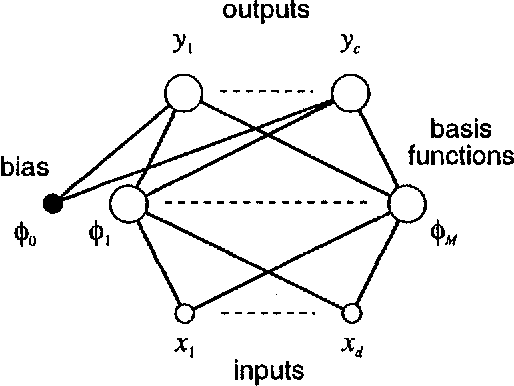
\includegraphics[width=0.5\textwidth]{bishopnn.png}
    \caption{Courtesy of C. Bishop (1995)}
    \label{fig:bishopnn}
\end{figure}

\subsection{Methodology}

The ARDL Bounds Test confirmed that our variable selection was sensible by virtue
of its establishment of cointegration. The RBF-NN, it is hoped, will be able
to capture intricate non-linear patterns in the data that the econometric model
was unable to, and accordingly be able to predict with accuracy the future price
movements. The RBF-NN was utilised for both short-term and long-term 
predictions. For short-term forecasting, 
the model was tested over a 5-month horizon, based on the recommendation of the
ARDL model, while the long-term predictions spanned 57 months. 
We differenced the data based on the recommendations of the 
unit root tests conducted earlier to achieve stationarity. 

We began by normalising the data, using a z-score normalisation. This is because
neural networks work best with data
that is between a specified range; it ensures that the data is roughly uniformly
distributed between the network inputs and outputs 
(Mendelsohn, 1993, Preprocessing Data for Neural Networks). Following this 
we had to program the RBF-NN into Python. As no specific RBF package exists
in Python, we used the kernel regression approach outlined by 
Bishop, using the GaussianProcessRegressor (GPR) package in Python.

\subsubsection{The Gaussian Process Regressor}

The Scikit GaussianProcessRegressor is based on the 
standard linear regression 
model, equipped with Gaussian noise,

\begin{align} 
    f(x) = x^{T}w, \quad{y = f(x) + \varepsilon}
\end{align}

where $y$ differs from the function values $f(x)$ by noise which is assumed
to follow an independent and identically distributed Gaussian distribution
$\mathcal{N}_1$
\begin{align*}
    \varepsilon \sim \mathcal{N}_1 \bigl(0, \sigma_{n}^2\bigr)
\end{align*}
This assumption together with the model produces the 
probability density of the observations given the inputs, 
which is factored over cases in the training set, 
permissible because of the independence assumption,

\begin{align}
    p(y|X,w) = \prod_{i=1}^{n} p(y_i|x_i ,w) = \mathcal{N}\bigl(X^T, \sigma_{n}^2 I\bigr)
\end{align}

As this is a Bayesian model we need to specify a \textit{prior distribution} over the parameters, 
expressing our beliefs about the prior
parameters before we examine the observations. A covariance function or kernel
is specified according to the characteristics of the data; in our model this 
is the generalised inverse multiquadric

$$ k(x,x') = \biggl( ||x-x'|| + \sigma^2\biggr)^{-\beta} $$
and used to construct the covariance matrix $K$, which along with 
a mean of $0$ forms the distribution of the the weights 
$$ w \sim \mathcal{N}\bigl(0, K\bigr)$$
By Bayes' Theorem, 

\begin{align}
    p(w|y, X) = \frac{p(y|X,w) p(w)}{p(y|X)}
\end{align}
Using this, the posterior distribution is then obtained

\begin{align}
    p(w|y, X) \sim \mathcal{N}\bigl(\frac{A^{-1}Xy}{\sigma_{n}^{2}}, A^{-1}\bigr)
\end{align}
where the covariance matrix $A^{-1} = K^{-1} + \frac{XX^T}{\sigma_{n}^2}$.
To make predictions on a test case all possible $w$
values, weighted by their posterior probability, are averaged to obtain the
predictive distribution, upon which predicted outputs are computed.

\subsubsection{The Network}

A $4$-dimensional input space $X$
passes inputs $\boldsymbol{\mathrm{x}}_1, \boldsymbol{\mathrm{x}}_2,\ldots \boldsymbol{\mathrm{x}}_{n}$
and corresponding outputs \( y = \{y_1, y_2, \dots, y_n\} \), through the first
layer, in which the covariance function $(x,x')$
is applied, the goal being to determine the distribution of the weights. Prior to this,
the optimal hyperparameters in the covariance function, which plays an analogous
role to the RBF basis function, are calculated using GridSearch Cross Validation; these hyperparameters are:
\begin{enumerate}
    \item $\alpha$: a regularisation parameter which represents a small quantity
    that is added to the diagonals of the covariance matrix to ensure it is 
    invertible. 
    \item $\beta$: the power in the covariance function, which controls the shape of the function.
    \item $\sigma$: a parameter which controls how much of the noise in the data the kernel accounts for; naturally, 
    it moderates the risk of overfitting and underfitting.
    \item Length scale: a parameter that controls the influence - analogous to 
    the width each RBF neuron possesses - that each kernel (analogous to node) is to have.
\end{enumerate}
following this the model uses the training observation $(y,X)$ to find
the posterior predictive distribution, and with it the predicted output, after 
averaging over all possible $w$, weighted by their likelihood according to (10). 

\subsection{Results}

The model returned a mean absolute error of MAE $=0.16$ and 
$R^2 = 9\%$ for the long term prediction, outperforming the ARDL-Error Correction model by 
$2.4\%$.


\begin{figure}[h]
    \centering
    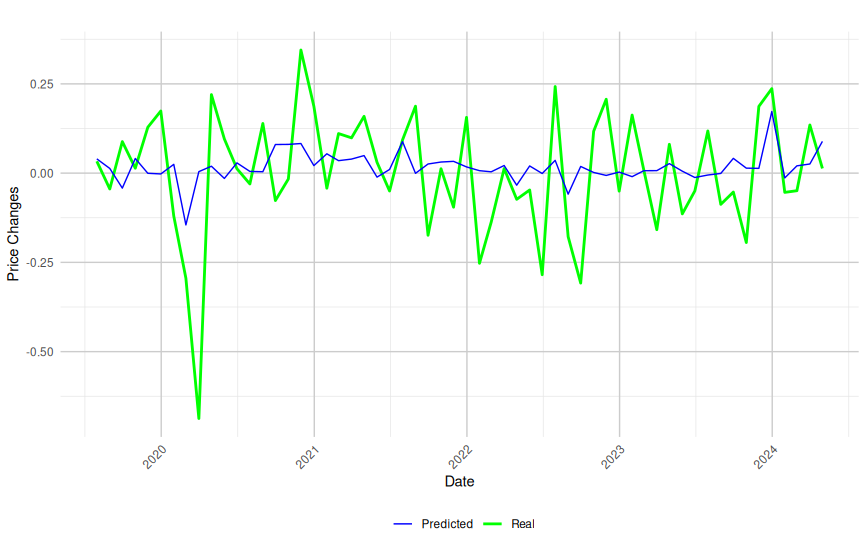
\includegraphics[width=0.8\textwidth]{long-term-monthly.png}
    \caption{Long-term predicted vs monthly real FTSE250 price changes}
    \label{fig:lmonthly}
\end{figure}

The interpretation of this is that, historically, the variations in the 
Consumer Price Index, interest rate, USD/GBP exchange rate, and M3 money 
supply have explained or accounted for $9\%$ of the fluctuations of the
FTSE250 value; in the context of a phenomenon as complex as the stock market,
which is influenced by an inumerable quantity of factors such as investor sentiment
- inherently irrational, 
political instability, geopolitical shocks, corporate governance, and financial regulation, this is 
unsurprising. Furthermore, the selection of economic variables in this study
is by no means exhaustive; commodity prices, international trade dynamics,
economic growth, and many other variables also exert a non-insignificant 
effect on the stock market.


The short-term prediction yielded MAE = $0.07$ and 
$R^2 = 61\%$, for a 5-month time horizon.
The significantly better performance of the model in the short-run
indicates that the selected macroeconomic variables possesses
a stronger predictive power over shorter periods. This was highlighted 
earlier in the ARDL model, with the interest rate and money supply significantly
impacting the FTSE250 price. 

In the short-term, which we define as 5 months, 
as per the optimum lag for the FTSE250 in the ARDL model, the market movements
are more closely tied to recent deviations in the economy, because theoretically
the short-run is not exposed to the various unforeseen external shocks and structural changes
that dilute the relationship between these variables and the stock market in the 
long-run. Essentially, as we stretch our prediction window, we 
introduce more uncertainty and unknowns, which translates into a 
lower predictive quality.

\begin{figure}[h]
    \centering
    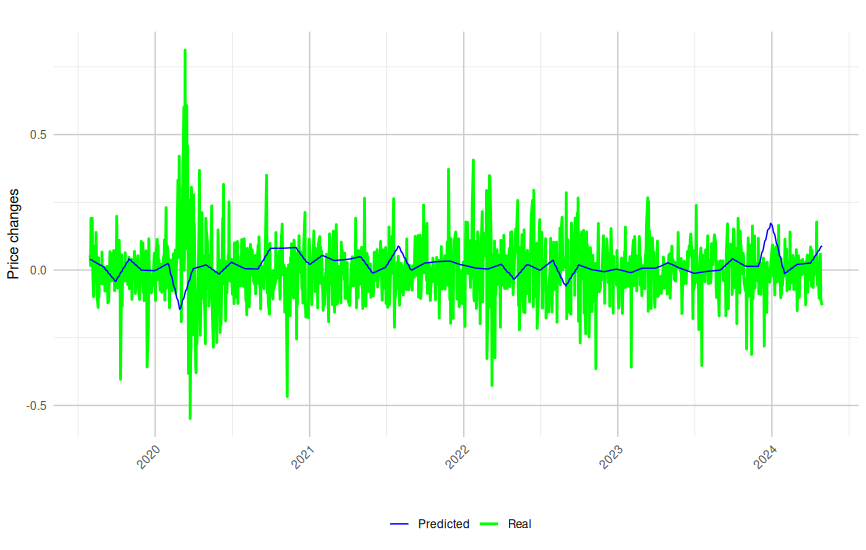
\includegraphics[width=0.8\textwidth]{long-term-daily.png}
    \caption{Long-term predicted vs daily real FTSE250 price changes}
    \label{fig:ldaily}
\end{figure}

Furthermore, as the time horizon extends into the long-run, fundamental factors 
begin to matter a lot more. The compound effect of earnings, cash flows and
managerial efficiencies begins to outweigh the 
influence of fluctuating macroeconomic sentiment. Thus, in the long-term
we see a different picture altogether.

\begin{figure}[h]
    \centering
    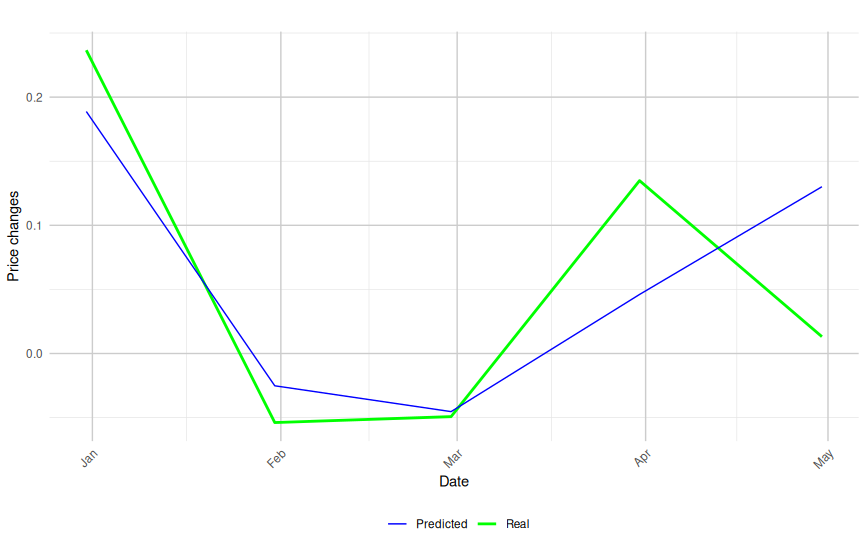
\includegraphics[width=0.8\textwidth]{short-term-monthly.png}
    \caption{Short-term predicted vs monthly real FTSE250 price changes}
    \label{fig:smonthly}
\end{figure}

\begin{figure}[h]
    \centering
    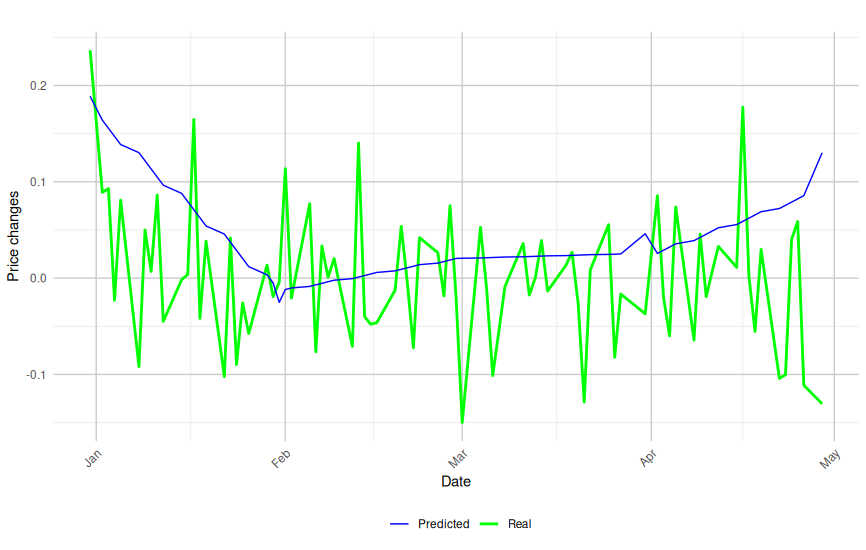
\includegraphics[width=0.8\textwidth]{short-term-daily.png}
    \caption{Short-term predicted vs daily real FTSE250 price changes}
    \label{fig:sdaily}
\end{figure}

\section{Conclusion}

This study first tested the findings of previous econometric research on the 
UK stock market, relating the impact of some especially
relevant macroeconomic factors on the FTSE250. 

Stock markets provide important information on the economy, 
and economic policymakers are vigilant in tracking the fluctuations 
in these markets, and try to forecast the 
forthcoming fluctuations based on policy changes that affect the macroeconomy.
Within this context, the study examined the 
impacts of the interest rate, USD/GBP
exchange rate, the consumer price index, and 
M3 money supply market activity on
the FTSE250 index over the October 1993 – April 2024 period.
The results suggest a cointegrated long-run
relationship between the macroeconomic variables and the stock market index. 
The long-run coefficients imply that
increases in the interest rate and depreciation in the exchange rate
significantly depress the FTSE250 value. 
Policymakers dealing with forecasting the UK stock markets
should consider the factors in the study, and to raise the stock
market's value, a lower interest rate regime should be adopted and 
the Pound should be made more competitive.

The the study also investigated the efficacy of machine learning methods in 
the field of stock-econometric forecasting, and returned good results, providing investors
with an accurate short-term forecast tool, and also providing economists
with a quantitative non-econometric measure of the 
long-term influence of the selected macroeconomic 
variables on the FTSE250 that outperforms a standard econometric model.

Further research should endeavour to include other macroeconomic variables such as 
foreign direct and portfolio investment, commodity prices and economic growth.
Falling outside the immediate scope of the current study, 
an autoregresive model could also be tried, including the past values of the 
FTSE250 in the input space to provide a more accurate model. In addition, 
a more granular data set could be utilised by applying a 
Brownian bridge algorithm to generate daily macroeconomic data and 
subsequently testing the RBF-NN against other neural networks 
such as auto-regressive LSTMs and GRUs, as well as other machine learning methods suited for 
forecasting such as Support Vector Machines (SVM). 

\bibliographystyle{plainnat}
\bibliography{paper}

\end{document}
